\documentclass{article}
\usepackage{tikz}
\usepackage{ctex}
\usepackage{booktabs}
\usepackage{bm}
\usepackage{indentfirst}
\usepackage{graphicx} 
\usepackage[export]{adjustbox} 
\usepackage{float}
\usepackage{amsmath}
\usepackage{amsfonts}
\usepackage{lmodern}
\usepackage{geometry}
\usepackage{color}
\usepackage{hyperref}
\def\mark{\textcolor{red}}
\geometry{a4paper, left=2cm, right=2cm, top=3cm, bottom=3cm}
\setlength{\parindent}{2em}
\linespread{1.5}


\begin{document}

\title{服务器使用指南}
\author{刘雷轶男\quad 智朝晖}
\maketitle

\begin{abstract}
这是一篇介绍组内服务器如何使用的指南。本文的源代码放在了\href{https://www.overleaf.com/}{Overleaf}上,有错误或过时的信息
请大家及时更新。如果有不详尽的地方,请及时指出。希望大家多提建议。
\end{abstract}
\newpage

\tableofcontents
\newpage

\section{服务器基本信息}
目前组内一共有四台服务器,它们都配备了双路6238R,Centos7系统,基本信息如下所示,其中编号2配有GPU。

\begin{table}[H]\label{info}
    \centering
    \begin{tabular}{|c|c|c|c|c|c|c|}
    \hline
    编号 & 所在楼层 & IP地址           & 端口 & 配置的软件          & 管理人  & 内存大小    \\ \hline
    1  & 8楼   & 172.17.176.141 & 88 & Matlab, Python & 崔健    & 188T \\ \hline
    2  & 8楼   & 172.17.176.141 & 2  & Matlab, Python & 崔健    & 1.5T \\ \hline
    3  & 8楼   & 172.17.177.238 & 22 & Matlab, Python & 王京京  &  188G    \\ \hline
    4  & 6楼   & 172.17.162.3   & 22 & Matlab, Python, Julia  & 刘雷轶男 & 754G \\ \hline
    \end{tabular}
\end{table}

目前服务器的管理员是刘雷轶男。
如果对在Mac OS系统上使用服务器,或对linux系统,亦或是在服务器上使用Python有疑问,可以找刘雷轶男\footnote{微信:liuleiyinan\_buaa}讨论。
如果对在Windows系统上使用服务器,或者是对服务器上Matlab、Julia使用有疑问,可以找智朝晖\footnote{微信:z2276780832}讨论。

\section{如何连接服务器}
\subsection{MacOS系统}
对于MacOS系统,可以通过以下方式连接服务器:
\begin{enumerate}
    \item 同时按一下command键和空格键打开聚焦搜索,输入terminal,按回车,然后会出现终端界面
    \item 输入\quad \verb|ssh -p 端口号 用户名@IP地址|\quad 后回车
    \begin{figure}[H]
        \centering
        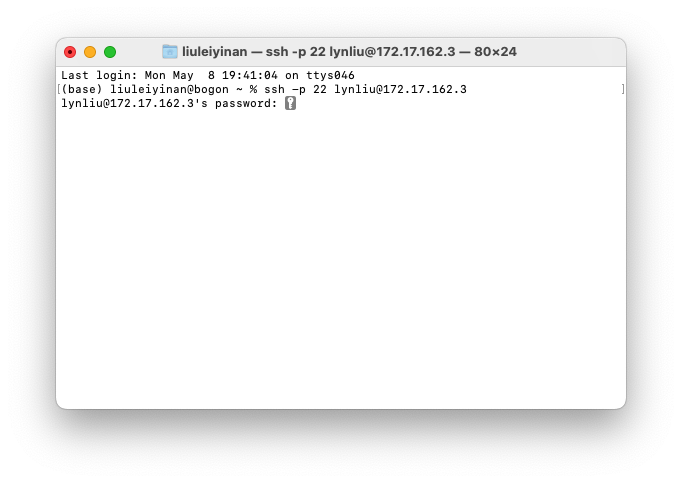
\includegraphics[scale = 0.5]{figs/1.png}
    \end{figure}
    \item 输入密码后,回车,便成功登录上了服务器
    \begin{figure}[H]
        \centering
        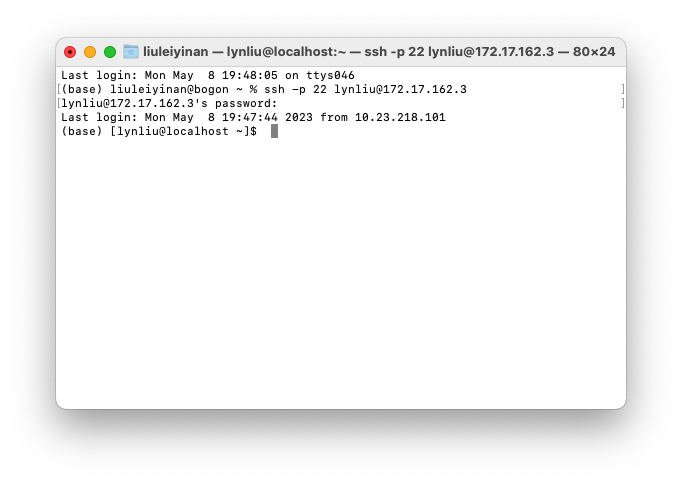
\includegraphics[scale = 0.5]{figs/2.png}
    \end{figure}
\end{enumerate}

\subsection{Windows系统}
对于Windows系统,可以通过和上文MacOS系统一样,通过ssh命令连接服务器,但这里我们更推荐用具有ssh服务同时还可以进行文件管理和传输的软件,比如Xshell和MobaXterm。下面我们以MobaXterm为例,其官网为\url{https://mobaxterm.mobatek.net/}:

\begin{enumerate}
    \item 在左上角部分菜单栏选择Session,即建立一个联系/对话。如图\ref{fig6}
    \begin{figure}[H]
    \centering
    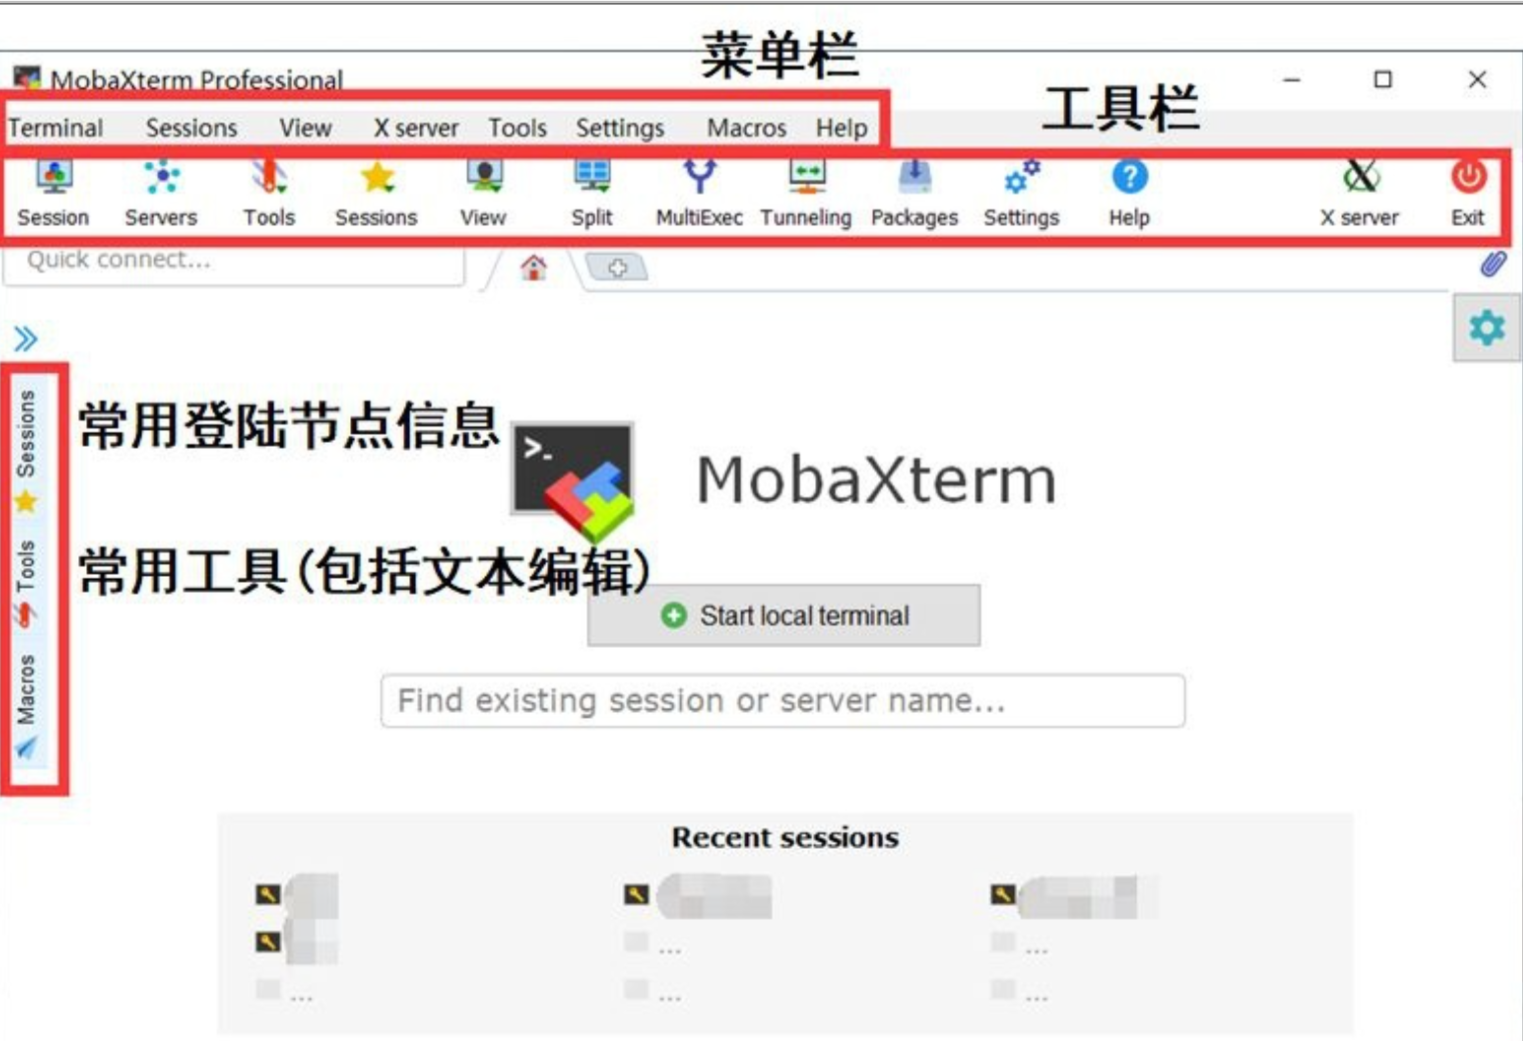
\includegraphics[scale=0.3]{figs/6.png}
    \caption{MobaXterm选择页面}
    \label{fig6}
    \end{figure}
    \item 选择SSH连接方式,在Basic SSH settings部分填入远程ip(内网ip或者是校园网ip),然后填入用户名,选择相应端口,(具体信息参见\ref{info}), 点OK就可以了。
    \begin{figure}[H]
    \centering
    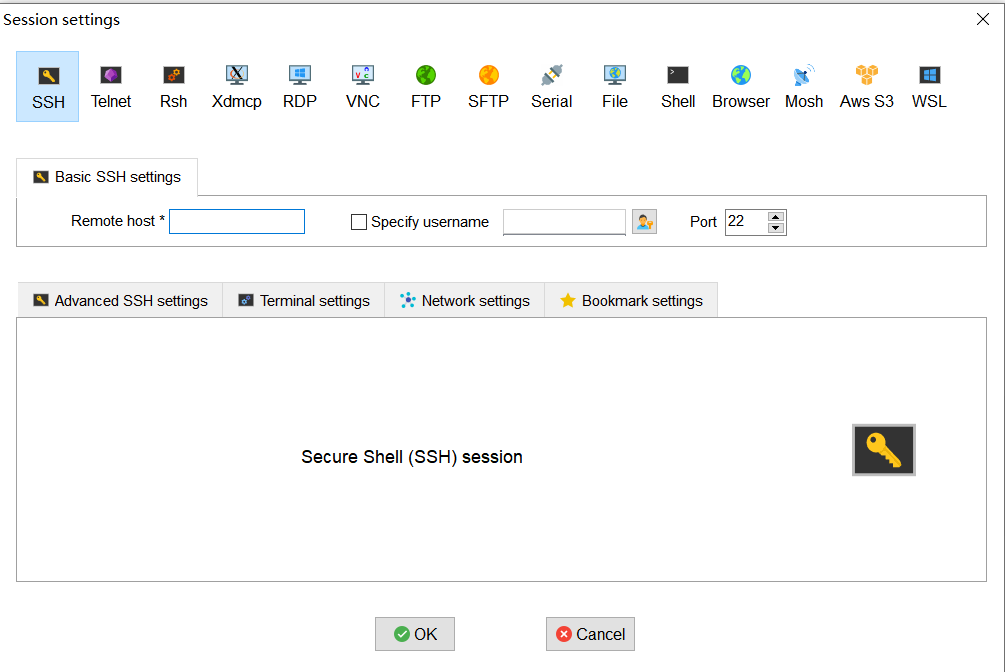
\includegraphics[scale=0.5]{figs/7.png}
    \caption{新建ssh会话}
    \label{fig7}
\end{figure}
    \item 会显示\mark{login as:},输入用户名后,敲回车即成功进入。
    \begin{figure}[H]
        \centering
        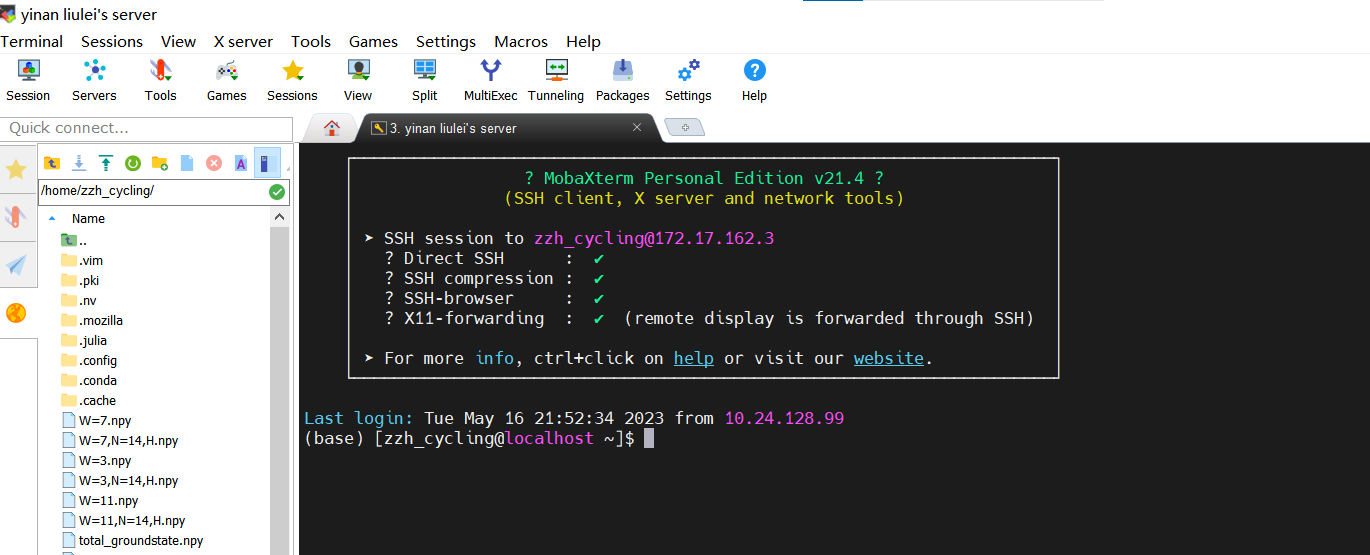
\includegraphics[scale=0.4]{figs/8.png}
    \end{figure}
\end{enumerate}


\section{Linux系统的基本操作}
常用的命令,包括:
\begin{itemize}
    \item 切换目录 \verb|cd| ; 切换到上一级目录 \verb|cd ..| ; 回到当前账号的工作目录 \verb|cd ~|
    \item 查看目录 \verb|ls| ; 列出文件详细信息 \verb|ls -l| ; 列出当前目录下所有文件(包括隐藏的)\verb|ls -a|
    \item 创建目录 \verb|mkdir|
    \item 查看文件 \verb|cat|
    \item 删除文件 \verb|rm| ; 删除目录 \verb|rm -r| ; 强制删除 \verb|rm -f|
    \item 显示当前目录 \verb|pwd|
    \item 动态显示当前耗费资源最多进程信息 \verb|top|
    \item 显示瞬间进程状态 \verb|ps| , 比如查看所有python程序的运行情况
    \begin{figure}[H]
        \centering
        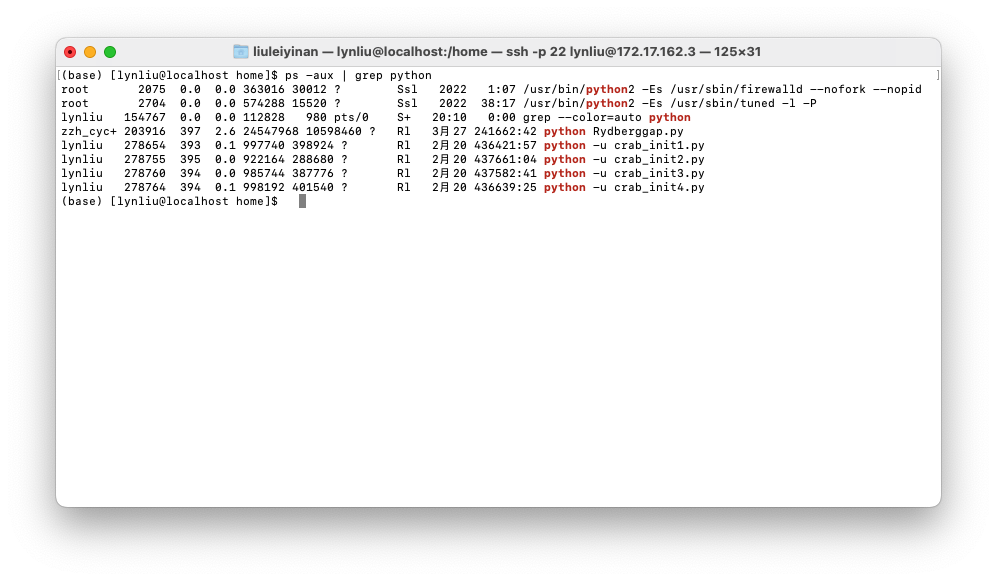
\includegraphics[scale = 0.3]{figs/3.png}
        \caption{查看所有python程序的运行情况,grep表示筛选有python关键字的进程名}
    \end{figure}
    \item 命令帮助 \verb|man| , 比如\verb|grep|命令不会用,输入\verb|man grep|看文档
    \item 清屏 \verb|clear|
    \item 杀死进程 \verb|kill|
    \item 查看硬盘使用情况 \verb|df -h|
    \item 移动文件位置 \verb|mv /xxx/xxx /xxx/|
\end{itemize}

\section{文件管理与传输}
\subsection{MacOS系统}
对于MacOS系统,可以使用Cyberduck等其他远程文件管理软件。
Cyberduck的官网下载地址为\url{https://cyberduck.io/download/}。

下面介绍Cyberduck如何使用。
\begin{enumerate}
    \item 在书签页面,右键点击,选择新建书签
    \item 如下图一样配置即可,\mark{第一栏一定要选成SFTP},名称和备注名可任选,服务器、端口按上面的表填写即可。
    \begin{figure}[H]
        \centering
        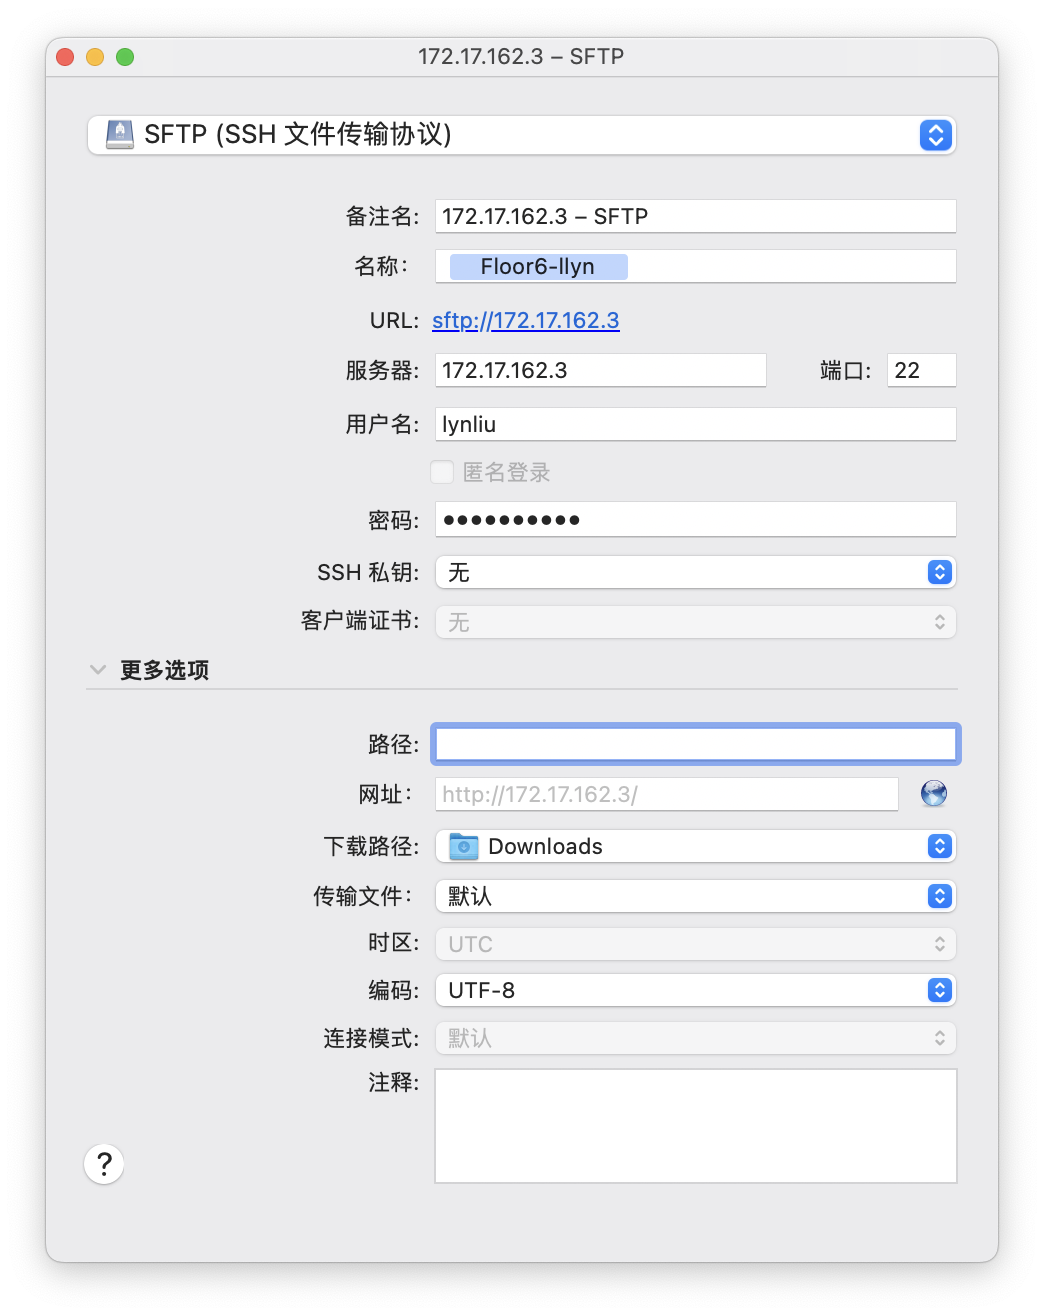
\includegraphics[scale = 0.5]{figs/4.png}
        \caption{配置书签}
    \end{figure}
    \item 创建完成后,双击创建的书签,就可以连接到服务器了,后续的操作都是可视化的。
\end{enumerate}

\subsection{Windows系统}
Windows系统下的远程文件管理和传输也可以用Xshell和MobaXterm,这里接着以MobaXterm为例:

在MobaXterm里上传与下载文件十分方便,只需要在本地和MobaXterm页面之间进行拖拽即可,或者采用鼠标右键选择相应的下载功能。

\section{Matlab使用指南}
如果用MobaXterm连接服务器的话,直接在命令行输入matlab,然后根据xmanager工具可以在本地打开matlab的界面工具,实现本地直接编写matlab代码并运行。

如果想用命令行操作的话,假设文件名为matlabfile.m,进入m文件所在目录后,运行

\verb|matlab -nodesktop -nosplash -rmatlabfile|
\section{Python使用指南}
所有的服务器上都装有anaconda,python的版本都在3.9及以上,并且base环境装了常用的库,包括:
\begin{itemize}
    \item numpy: \url{https://numpy.org}
    \item scipy: \url{https://scipy.org}
    \item matplotlib: \url{https://matplotlib.org}
    \item qutip: \url{https://qutip.org}
\end{itemize}
如果需要可以自行安装其他的包,如果安装失败请联系管理员安装。
由于只有\verb|root|权限才可以新建环境,如果需要创建新环境也需要联系管理员。
\subsection{导入conda路径}
在拿到账号密码后,要和管理员确认是否将该账号加入了anaconda的用户组,如果不在该用户组里,以下的操作是无效的。
可以使用\verb|groups|命令查看目前账号是否在anaconda用户组中。
\begin{figure}[H]
    \centering
    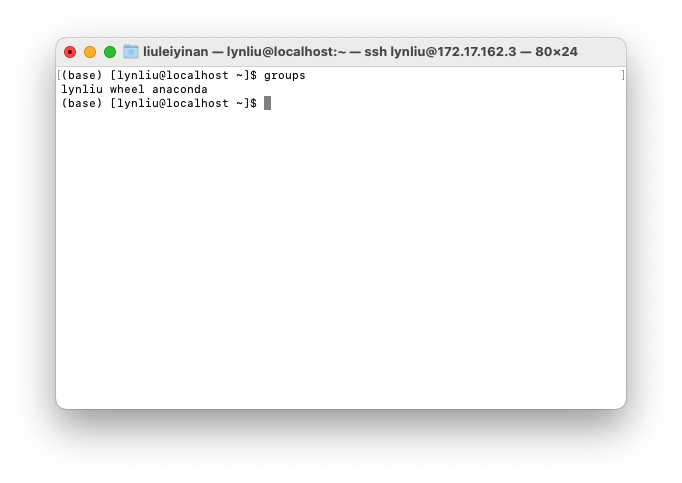
\includegraphics[scale = 0.5]{figs/5.png}
    \caption{如果在anaconda用户组里,会出现anaconda名称}
\end{figure}
确认之后,登录账号,输入\verb|cd ~|,确保当前在该账号的主目录下,更改\verb|.bashrc|文件的配置。将\verb|.bashrc|
文件的内容改为
\begin{verbatim}
if [ -f /etc/bashrc ]; then
 . /etc/bashrc
fi
__conda_setup="$('/usr/local/anaconda3/bin/conda' 'shell.bash' 'hook' 2> /dev/null)"
if [ $? -eq 0 ]; then
    eval "$__conda_setup"
else
    if [ -f "/usr/local/anaconda3/etc/profile.d/conda.sh" ]; then
        . "/usr/local/anaconda3/etc/profile.d/conda.sh"
    else
        export PATH="/usr/local/anaconda3/bin:$PATH"
    fi
fi
unset __conda_setup
\end{verbatim}
或者在本地创建一个包含上述内容的txt文件,通过Cyberduck、Xshell等工具上传到服务器上再改名为\verb|.bashrc|也可。
修改完成后,输入\verb|logout|退出登录,再次登录时,就可以直接使用conda和python命令了。

更改完后可以使用\verb|cat .bashrc|查看是否更改成功。
\subsection{运行python文件}
将python上传到服务器上后,进入该文件所在目录,输入
\verb|python xxx.py|
即可运行该程序。

如果程序运行时间较长,想让程序在退出登录后继续运行,可以使用\verb|nohup|命令
\begin{verbatim}
    nohup python -u xxx.py >output.log 2>&1 &
\end{verbatim}
其中\verb|xxx.py|是所运行的文件,\verb|output.log|是\verb|xxx.py|运行时输出内容的存放文件。
如果\verb|xxx.py|出现错误,或者意外退出,信息都会保存在\verb|output.log|中。

服务器可以一次提交多个python程序。

\subsection{注意事项}
Python程序本身是只能单核运行的,但是如果使用numpy和scipy库,此时它们调用的mkl会多线程运行,从而占据许多CPU资源,
并且此时的程序运行效率大大下降。因此,在服务器上运行python程序时,务必在运行的python脚本开头加上如下代码
\begin{verbatim}
    import os
    os.environ["MKL_NUM_THREADS"] = "2"
\end{verbatim}
这样,程序的运行就不会有很高的CPU占用率了,如果设置为``2'',则最高应只有$200\%$的占用率。此处的具体数字
可以根据程序的运算量灵活设置,最好不要一次性占用太多CPU资源。

\subsection{终止python程序}
如果想要中断某个python程序的运行,
可以使用
\begin{verbatim}
    ps -aux | grep python
\end{verbatim}
列出所有的python程序,找到你想终止的程序的PID后,输入
\begin{verbatim}
    kill xxxxxxxx
\end{verbatim}
回车即可。(\verb|xxxxxxxx|表示某一PID)

\section{Julia使用指南}
由于Julia仍属于十分小众的语言,所以只在一台服务器上安装了Julia(具体见服务器基本信息),版本号是\verb|1.8.5|。
如果要使用Julia,请在\verb|.bashrc|文件中加入以下路径:
\begin{verbatim}
    export PATH="/data/julia-1.8.5/bin:$PATH"
\end{verbatim}
更改\verb|.bashrc|文件后,重新登录账号或者用\verb|source .bashrc|刷新一下后,就可以用\verb|julia|
直接进入Julia REPL了。

\subsection{运行Julia}
运行Julia程序的步骤与python是类似的
\begin{verbatim}
    nohup julia xxx.jl >output.log 2>&1 &
\end{verbatim}
即可在后台持续运行\verb|xxx.jl|程序,并将输出或报错信息记录在\verb|output.log|中。服务器可以一次提交多个Julia程序。
\subsection{将Julia链接到MKL库上}
因为Julia默认是链接到OpenBLAS库上,而在Intel芯片上MKL运行更有效率更高效,所以你可以选择将Julia的LinearAlgebra的线性代数库换成MKL,操作如下:

\begin{enumerate}
    \item 进入Julia REPL后,\verb|using Pkg; Pkg.add("MKL")|
    \item 然后在程序导入库的\mark{第一行}写上:
    \verb|using MKL|,就能愉快地用MKL来计算了。\\
    (虽然这时候你输入\verb|using LinearAlgebra|;然后
    \verb|LinearAlgebra.BLAS.get_config()|;\\或者\verb|LinearAlgebra.BLAS.vendor()|还是显示的OpenBLAS)
\end{enumerate}

\section{使用GPU加速计算}
使用GPU加速计算基本都是利用商业公司已经写好的计算架构和GPU计算库来编程,使用GPU加速计算有两种方法:
\begin{enumerate}
    \item 直接使用CUDA的C/C++版本进行编程。
    \item Python使用Numba库调用CUDA,或者使用cupy,或者是Pytorch等已经生态很良好的深度学习框架来编写程序。
\end{enumerate}

\section{硬盘使用}
如果有很大的文件需要储存,建议移动到硬盘中储存。
目前一般在\verb|/data|或\verb|/data1|下储存大文件。下面是操作步骤。
(如果有服务器没有开启权限,请联系管理员。)
\begin{enumerate}
    \item 如果需要将文件存到硬盘中,需先创建一个以自己用户名为文件名的文件夹。
    切换到\verb|/data|路径下:\verb|cd /data|,然后创建文件夹:\verb|mkdir 用户名|。
    \item 将文件移动到该路径下:
    \begin{verbatim}
        mv 原先文件路径 新的路径
    \end{verbatim}
    比如:
    \begin{verbatim}
        mv /home/lynliu/xxx.txt /data/lynliu/
    \end{verbatim}
\end{enumerate}

\end{document}